
%% bare_conf_compsoc.tex
%% V1.4b
%% 2015/08/26
%% by Michael Shell
%% See:
%% http://www.michaelshell.org/
%% for current contact information.
%%
%% This is a skeleton file demonstrating the use of IEEEtran.cls
%% (requires IEEEtran.cls version 1.8b or later) with an IEEE Computer
%% Society conference paper.
%%
%% Support sites:
%% http://www.michaelshell.org/tex/ieeetran/
%% http://www.ctan.org/pkg/ieeetran
%% and
%% http://www.ieee.org/

%%*************************************************************************
%% Legal Notice:
%% This code is offered as-is without any warranty either expressed or
%% implied; without even the implied warranty of MERCHANTABILITY or
%% FITNESS FOR A PARTICULAR PURPOSE! 
%% User assumes all risk.
%% In no event shall the IEEE or any contributor to this code be liable for
%% any damages or losses, including, but not limited to, incidental,
%% consequential, or any other damages, resulting from the use or misuse
%% of any information contained here.
%%
%% All comments are the opinions of their respective authors and are not
%% necessarily endorsed by the IEEE.
%%
%% This work is distributed under the LaTeX Project Public License (LPPL)
%% ( http://www.latex-project.org/ ) version 1.3, and may be freely used,
%% distributed and modified. A copy of the LPPL, version 1.3, is included
%% in the base LaTeX documentation of all distributions of LaTeX released
%% 2003/12/01 or later.
%% Retain all contribution notices and credits.
%% ** Modified files should be clearly indicated as such, including  **
%% ** renaming them and changing author support contact information. **
%%*************************************************************************


% *** Authors should verify (and, if needed, correct) their LaTeX system  ***
% *** with the testflow diagnostic prior to trusting their LaTeX platform ***
% *** with production work. The IEEE's font choices and paper sizes can   ***
% *** trigger bugs that do not appear when using other class files.       ***                          ***
% The testflow support page is at:
% http://www.michaelshell.org/tex/testflow/



\documentclass[conference,compsoc]{IEEEtran}
% Some/most Computer Society conferences require the compsoc mode option,
% but others may want the standard conference format.
%
% If IEEEtran.cls has not been installed into the LaTeX system files,
% manually specify the path to it like:
%\documentclass[conference,compsoc{/Users/czxpc/Documents/shared/report/Report/latex/Sty/IEEEtran}


%Added by Zhixuan Cao to make reference more compact
\def\IEEEbibitemsep{0pt plus .6pt}



% Some very useful LaTeX packages include:
% (uncomment the ones you want to load)


% *** MISC UTILITY PACKAGES ***
%
%\usepackage{ifpdf}
% Heiko Oberdiek's ifpdf.sty is very useful if you need conditional
% compilation based on whether the output is pdf or dvi.
% usage:
% \ifpdf
%   % pdf code
% \else
%   % dvi code
% \fi
% The latest version of ifpdf.sty can be obtained from:
% http://www.ctan.org/pkg/ifpdf
% Also, note that IEEEtran.cls V1.7 and later provides a builtin
% \ifCLASSINFOpdf conditional that works the same way.
% When switching from latex to pdflatex and vice-versa, the compiler may
% have to be run twice to clear warning/error messages.






% *** CITATION PACKAGES ***
%
\ifCLASSOPTIONcompsoc
  % IEEE Computer Society needs nocompress option
  % requires cite.sty v4.0 or later (November 2003)
  \usepackage[nocompress]{cite}
\else
  % normal IEEE
  \usepackage{cite}
\fi
% cite.sty was written by Donald Arseneau
% V1.6 and later of IEEEtran pre-defines the format of the cite.sty package
% \cite{} output to follow that of the IEEE. Loading the cite package will
% result in citation numbers being automatically sorted and properly
% "compressed/ranged". e.g., [1], [9], [2], [7], [5], [6] without using
% cite.sty will become [1], [2], [5]--[7], [9] using cite.sty. cite.sty's
% \cite will automatically add leading space, if needed. Use cite.sty's
% noadjust option (cite.sty V3.8 and later) if you want to turn this off
% such as if a citation ever needs to be enclosed in parenthesis.
% cite.sty is already installed on most LaTeX systems. Be sure and use
% version 5.0 (2009-03-20) and later if using hyperref.sty.
% The latest version can be obtained at:
% http://www.ctan.org/pkg/cite
% The documentation is contained in the cite.sty file itself.
%
% Note that some packages require special options to format as the Computer
% Society requires. In particular, Computer Society  papers do not use
% compressed citation ranges as is done in typical IEEE papers
% (e.g., [1]-[4]). Instead, they list every citation separately in order
% (e.g., [1], [2], [3], [4]). To get the latter we need to load the cite
% package with the nocompress option which is supported by cite.sty v4.0
% and later.





% *** GRAPHICS RELATED PACKAGES ***
%
\ifCLASSINFOpdf
  \usepackage[pdftex]{graphicx}
  % declare the path(s) where your graphic files are
  % \graphicspath{{../pdf/}{../jpeg/}}
  % and their extensions so you won't have to specify these with
  % every instance of \includegraphics
  % \DeclareGraphicsExtensions{.pdf,.jpeg,.png}
\else
  % or other class option (dvipsone, dvipdf, if not using dvips). graphicx
  % will default to the driver specified in the system graphics.cfg if no
  % driver is specified.
  % \usepackage[dvips]{graphicx}
  % declare the path(s) where your graphic files are
  % \graphicspath{{../eps/}}
  % and their extensions so you won't have to specify these with
  % every instance of \includegraphics
  % \DeclareGraphicsExtensions{.eps}
\fi
% graphicx was written by David Carlisle and Sebastian Rahtz. It is
% required if you want graphics, photos, etc. graphicx.sty is already
% installed on most LaTeX systems. The latest version and documentation
% can be obtained at: 
% http://www.ctan.org/pkg/graphicx
% Another good source of documentation is "Using Imported Graphics in
% LaTeX2e" by Keith Reckdahl which can be found at:
% http://www.ctan.org/pkg/epslatex
%
% latex, and pdflatex in dvi mode, support graphics in encapsulated
% postscript (.eps) format. pdflatex in pdf mode supports graphics
% in .pdf, .jpeg, .png and .mps (metapost) formats. Users should ensure
% that all non-photo figures use a vector format (.eps, .pdf, .mps) and
% not a bitmapped formats (.jpeg, .png). The IEEE frowns on bitmapped formats
% which can result in "jaggedy"/blurry rendering of lines and letters as
% well as large increases in file sizes.
%
% You can find documentation about the pdfTeX application at:
% http://www.tug.org/applications/pdftex





% *** MATH PACKAGES ***
%
\usepackage{amsmath}
% A popular package from the American Mathematical Society that provides
% many useful and powerful commands for dealing with mathematics.
%
% Note that the amsmath package sets \interdisplaylinepenalty to 10000
% thus preventing page breaks from occurring within multiline equations. Use:
\interdisplaylinepenalty=2500
% after loading amsmath to restore such page breaks as IEEEtran.cls normally
% does. amsmath.sty is already installed on most LaTeX systems. The latest
% version and documentation can be obtained at:
% http://www.ctan.org/pkg/amsmath





% *** SPECIALIZED LIST PACKAGES ***
%
\usepackage{algorithmic}
% algorithmic.sty was written by Peter Williams and Rogerio Brito.
% This package provides an algorithmic environment fo describing algorithms.
% You can use the algorithmic environment in-text or within a figure
% environment to provide for a floating algorithm. Do NOT use the algorithm
% floating environment provided by algorithm.sty (by the same authors) or
% algorithm2e.sty (by Christophe Fiorio) as the IEEE does not use dedicated
% algorithm float types and packages that provide these will not provide
% correct IEEE style captions. The latest version and documentation of
% algorithmic.sty can be obtained at:
% http://www.ctan.org/pkg/algorithms
% Also of interest may be the (relatively newer and more customizable)
% algorithmicx.sty package by Szasz Janos:
% http://www.ctan.org/pkg/algorithmicx




% *** ALIGNMENT PACKAGES ***
%
\usepackage{array}
% Frank Mittelbach's and David Carlisle's array.sty patches and improves
% the standard LaTeX2e array and tabular environments to provide better
% appearance and additional user controls. As the default LaTeX2e table
% generation code is lacking to the point of almost being broken with
% respect to the quality of the end results, all users are strongly
% advised to use an enhanced (at the very least that provided by array.sty)
% set of table tools. array.sty is already installed on most systems. The
% latest version and documentation can be obtained at:
% http://www.ctan.org/pkg/array


% IEEEtran contains the IEEEeqnarray family of commands that can be used to
% generate multiline equations as well as matrices, tables, etc., of high
% quality.




% *** SUBFIGURE PACKAGES ***
\ifCLASSOPTIONcompsoc
  \usepackage[caption=false,font=footnotesize,labelfont=sf,textfont=sf]{subfig}
\else
  \usepackage[caption=false,font=footnotesize]{subfig}
\fi
% subfig.sty, written by Steven Douglas Cochran, is the modern replacement
% for subfigure.sty, the latter of which is no longer maintained and is
% incompatible with some LaTeX packages including fixltx2e. However,
% subfig.sty requires and automatically loads Axel Sommerfeldt's caption.sty
% which will override IEEEtran.cls' handling of captions and this will result
% in non-IEEE style figure/table captions. To prevent this problem, be sure
% and invoke subfig.sty's "caption=false" package option (available since
% subfig.sty version 1.3, 2005/06/28) as this is will preserve IEEEtran.cls
% handling of captions.
% Note that the Computer Society format requires a sans serif font rather
% than the serif font used in traditional IEEE formatting and thus the need
% to invoke different subfig.sty package options depending on whether
% compsoc mode has been enabled.
%
% The latest version and documentation of subfig.sty can be obtained at:
% http://www.ctan.org/pkg/subfig




% *** FLOAT PACKAGES ***
%
\usepackage{fixltx2e}
% fixltx2e, the successor to the earlier fix2col.sty, was written by
% Frank Mittelbach and David Carlisle. This package corrects a few problems
% in the LaTeX2e kernel, the most notable of which is that in current
% LaTeX2e releases, the ordering of single and double column floats is not
% guaranteed to be preserved. Thus, an unpatched LaTeX2e can allow a
% single column figure to be placed prior to an earlier double column
% figure.
% Be aware that LaTeX2e kernels dated 2015 and later have fixltx2e.sty's
% corrections already built into the system in which case a warning will
% be issued if an attempt is made to load fixltx2e.sty as it is no longer
% needed.
% The latest version and documentation can be found at:
% http://www.ctan.org/pkg/fixltx2e


%\usepackage{stfloats}
% stfloats.sty was written by Sigitas Tolusis. This package gives LaTeX2e
% the ability to do double column floats at the bottom of the page as well
% as the top. (e.g., "\begin{figure*}[!b]" is not normally possible in
% LaTeX2e). It also provides a command:
%\fnbelowfloat
% to enable the placement of footnotes below bottom floats (the standard
% LaTeX2e kernel puts them above bottom floats). This is an invasive package
% which rewrites many portions of the LaTeX2e float routines. It may not work
% with other packages that modify the LaTeX2e float routines. The latest
% version and documentation can be obtained at:
% http://www.ctan.org/pkg/stfloats
% Do not use the stfloats baselinefloat ability as the IEEE does not allow
% \baselineskip to stretch. Authors submitting work to the IEEE should note
% that the IEEE rarely uses double column equations and that authors should try
% to avoid such use. Do not be tempted to use the cuted.sty or midfloat.sty
% packages (also by Sigitas Tolusis) as the IEEE does not format its papers in
% such ways.
% Do not attempt to use stfloats with fixltx2e as they are incompatible.
% Instead, use Morten Hogholm'a dblfloatfix which combines the features
% of both fixltx2e and stfloats:
%
 \usepackage{dblfloatfix}
% The latest version can be found at:
% http://www.ctan.org/pkg/dblfloatfix




% *** PDF, URL AND HYPERLINK PACKAGES ***
%
\usepackage{url}
% url.sty was written by Donald Arseneau. It provides better support for
% handling and breaking URLs. url.sty is already installed on most LaTeX
% systems. The latest version and documentation can be obtained at:
% http://www.ctan.org/pkg/url
% Basically, \url{my_url_here}.




% *** Do not adjust lengths that control margins, column widths, etc. ***
% *** Do not use packages that alter fonts (such as pslatex).         ***
% There should be no need to do such things with IEEEtran.cls V1.6 and later.
% (Unless specifically asked to do so by the journal or conference you plan
% to submit to, of course. )


% correct bad hyphenation here
\hyphenation{op-tical net-works semi-conduc-tor}


\begin{document}
%
% paper title
% Titles are generally capitalized except for words such as a, an, and, as,
% at, but, by, for, in, nor, of, on, or, the, to and up, which are usually
% not capitalized unless they are the first or last word of the title.
% Linebreaks \\ can be used within to get better formatting as desired.
% Do not put math or special symbols in the title.
\title{Data Management and Domain Adjusting Strategies for Implementing Parallel SPH Method in JPUE Simulation}


% author names and affiliations
% use a multiple column layout for up to three different
% affiliations
\author{\IEEEauthorblockN{Zhixuan Cao, Abani Patra, Matt Jones, ...}
\IEEEauthorblockA{Department of Mechanical and Aerospace Engineering\\
 The University at Buffalo\\
 Buffalo, New York 14260\\
Email: zhixuanc@buffalo.edu, abani@buffalo.edu}
%\and
%\IEEEauthorblockN{Homer Simpson}
%\IEEEauthorblockA{Twentieth Century Fox\\
%Springfield, USA\\
%Email: homer@thesimpsons.com}
%\and
%\IEEEauthorblockN{James Kirk\\ and Montgomery Scott}
%\IEEEauthorblockA{Starfleet Academy\\
%San Francisco, California 96678-2391\\
%Telephone: (800) 555--1212\\
%Fax: (888) 555--1212}
}
% conference papers do not typically use \thanks and this command
% is locked out in conference mode. If really needed, such as for
% the acknowledgment of grants, issue a \IEEEoverridecommandlockouts
% after \documentclass

% for over three affiliations, or if they all won't fit within the width
% of the page (and note that there is less available width in this regard for
% compsoc conferences compared to traditional conferences), use this
% alternative format:
% 
%\author{\IEEEauthorblockN{Michael Shell\IEEEauthorrefmark{1},
%Homer Simpson\IEEEauthorrefmark{2},
%James Kirk\IEEEauthorrefmark{3}, 
%Montgomery Scott\IEEEauthorrefmark{3} and
%Eldon Tyrell\IEEEauthorrefmark{4}}
%\IEEEauthorblockA{\IEEEauthorrefmark{1}School of Electrical and Computer Engineering\\
%Georgia Institute of Technology,
%Atlanta, Georgia 30332--0250\\ Email: see http://www.michaelshell.org/contact.html}
%\IEEEauthorblockA{\IEEEauthorrefmark{2}Twentieth Century Fox, Springfield, USA\\
%Email: homer@thesimpsons.com}
%\IEEEauthorblockA{\IEEEauthorrefmark{3}Starfleet Academy, San Francisco, California 96678-2391\\
%Telephone: (800) 555--1212, Fax: (888) 555--1212}
%\IEEEauthorblockA{\IEEEauthorrefmark{4}Tyrell Inc., 123 Replicant Street, Los Angeles, California 90210--4321}}




% use for special paper notices
%\IEEEspecialpapernotice{(Invited Paper)}



%The following package is added by Zhixuan Cao, I am not sure whether should I have %double line for IEEE computer society conference or not, need to make sure
%\usepackage{hhline} %to add double horizontal line in tabular

% make the title area
\maketitle

% As a general rule, do not put math, special symbols or citations
% in the abstract
\begin{abstract}
This paper presents a parallel implementation of smoothed particle hydrodynamics (SPH) method using the message passing interface (MPI) standard to simulate a turbulent jet or plume which is ejected from a nozzle into a uniform environment(JPUE). Background grid is used to reduce neighbors searching cost and decompose (redecompose) the domain. Space Filing Curve(SFC) based index is adopted to assign an unique identifier to each background grid. As simulation of JUPE requires adding of new particles during simulation, time-dependent SFC based indexes are assigned to particles to guarantee uniqueness of identifiers.  
%to distinguish particles added at the same position but different simulation time step. 
Both particle and background grid are managed by hashtables which ensure quick and flexible accessing, adding and deleting of element. %Additional link list attached to the hashtable is used to handle hash conflicts.
 A SFC based three dimensional domain decomposition and a dynamic load balancing strategy are implemented to ensure good load balance. In addition, computational domain is adjusted during simulation to reduce computational cost. 
Numerical tests show that our code has acceptable strong scalability and good weak scalability.
These strategies can be further applied to many other implementations of meshfree methods, especially those implementations that require irregular
particle distributions, adding and deleting of particles and leverage adaptive background grids.
\end{abstract}

% no keywords




% For peer review papers, you can put extra information on the cover
% page as needed:
% \ifCLASSOPTIONpeerreview
% \begin{center} \bfseries EDICS Category: 3-BBND \end{center}
% \fi
%
% For peerreview papers, this IEEEtran command inserts a page break and
% creates the second title. It will be ignored for other modes.
\IEEEpeerreviewmaketitle



\section{Introduction}
% no \IEEEPARstart
SPH (spherical particle hydrodynamics) is a meshless scheme, initially developed for astrophysical applications by Lucy\cite{lucy1977numerical} and Gingold and Monaghan\cite{gingold1977smoothed}. 
Subsequently it was extended to large strain solid mechanics and computational fluid mechanics. 
A lot of research has appeared  on  parallellization of SPH in the last few years. 
Goozee\cite{goozee2003distributed} implemented a simple SPH code using MPI, OpenMP and BSP. 
 Wenbo\cite{wenbo2014performance} presented a parallel SPH implementation on multi-core CPUs. 
  Holmes\cite{holmes2011framework} presented a simulation framework that enables distributed numerical computing in multi-core shared-memory environments. 
Dominguez\cite{dominguez2011optimization} presented optimizations for both CPU and GPU parallelization of a SPH method. 
 Ferrari\cite{ferrari2009new} parallelized a 3D SPH code using the message passing interface (MPI) standard, together with a dynamic load balancing strategy to improve the computational efficiency of the scheme. 
Kumar et. al. \cite{kumar2013parallel} implemented a parallel Godunov SPH in simulation of granular flows.
 Crespo\cite{crespo2015dualsphysics} used the GPUs to accelerate DualSPHysics by up to two orders of magnitude compared to the performance of the serial version.\\
However, most implementation of parallel SPH method presented to date are limited to standard SPH and benchmark problems like dam break, or relatively
 simple scenarios like breaking-waves, floodings etc. Work on more complicated problems, such as eruption of volcano plume which is essentially a mult-phase turbulent flow,
  ejection mixing process accompanied by microphysics phenomena like phase change of water, aggregation, reaction etc. is relatively rare. 
  Prediction of such  c complicated phenomena with acceptable accuracy at given time window requires resolutions (very high particle counts) that cannot been accomplished without parallel computing. What's more, imposing of some types of boundary conditions (such as realistic wind field, eruption boundary condition) requires dynamically adding and removing of particles during simulation. This requires efficient and more flexible data management scheme. What we need to point out is that the benefit of flexible data management strategies are not only limited to specific implementations of SPH. Actually, flexibility in data management are more critical for several advanced techniques of SPH, such as dynamic particle splitting techniques\cite{vacondio2012accurate, feldman2007dynamic}, which will give greater resolution at the area of interest by splitting one large particle to several smaller ones.
In this paper, we implement SPH to simulate a simplified version of complicated volcanic plume: the JPUE, and develop data management schemes for it.\\
Among existing CPU parallel SPH schemes, most of them focus on neighbors searching algorithm and dynamic load balancing. (eg.\cite{ferrari2009new, crespo2015dualsphysics}). Less attention has been paid to developing of more flexible data management schemes for more complicated problems. 
Fortunately, efficient and flexible data management strategies for high performance computing have been successfully implemented in mesh based methods (eg. \cite{laszloffy2000simple} for adaptive hp FEM, and \cite{pitman2003computing, patra2005parallel} for FVM). Motivated by techniques developed for mesh based methods, we present a complete framwork for parallelizing SPH program with MPI standard model allowing more flexible and efficient data access in this paper.\\
Any implementation of SPH code requires efficient searching and updating of neighbors during simulation. Of the many choices possible for this we adopted a background grid which was proposed by Monaghan and Lattanzio\cite{monaghan1985refined} and is quite popular in parallel SPH. The background grid is also used for domain decomposition in SPH. We refer to the elements of background grid, namely  squares for two dimension and cubics for three dimension, as buckets. 


As for the actual storage of data representing the physical quantities associated to each particle, different strategies  have been adopted in existing implementations of SPH. 
In both SPHysics\cite{dominguez2011optimization} and DualSPHysics\cite{crespo2015dualsphysics}, The physical quantities of each particle (position, velocity, density…) are stored in arrays, and the particles (and the arrays with particle data) are reordered following the order of the cells. This has two advantages: 1) access pattern is more regular and more efficient, 2) it is ease to identify the particles that belong to a cell by using a range since the first particle of each cell is known. But adding, deleting and especially accessing of particles are cumbersome.   Ferrari\cite{ferrari2009new} adopted linked lists using pointers so that particles can be deleted or added during the simulation. Storage problems caused by fix-size arrays are thereby also eliminated. We define C++ classes which contains all data of particle and bucket. As for the management of data, we adopt a hash table to store pointers to particles and buckets, which gives us not only flexibility of deleting and adding element, but also quicker access compared with linked list. Instead of using the "nature manner" to number particles, we adopt SFC based index to give each particle and background bucket an unique identifier -- a strategy known to preserve some locality at minimal cost. The SFC based numbering strategy is further extended to include time step information so that particles added at the same position but different time will have different identifiers. 

As for domain decomposition, even though more complicated graph-based partition tools\cite{biswas1999experiments} might get higher quality decomposition, they requires much more effort in programming and computation. So we adopt an easy-programming scheme based on SFC \cite{patra1999efficient}.\\
To the best of the author's knowledge, no implementation of SPH has the feature of adjusting computational domain based on simulation needs. For JPUE simulation, such feature will greatly reduce computational cost by avoiding computing of uninfluenced fluid. This feature is accomplished by adding a scan function to monitor the outermost layer of the domain and turn ghost particles to real particles at the proper time. 
%The computational cost of this additional scan function is low.
\\
The data structure, particle and bucket indexing strategies, domain decomposition , dynamic load balancing method and domain adjusting strategies in this paper can be easily adopted by other implementations of any meshfree methods(include SPH). The flexibility of data accessing enables implementing of meshless methods for solving of more complicated problems and using of more advanced techniques.\\
\section{Data Structure and Load Balance}
\begin{figure}[!t]
\centering
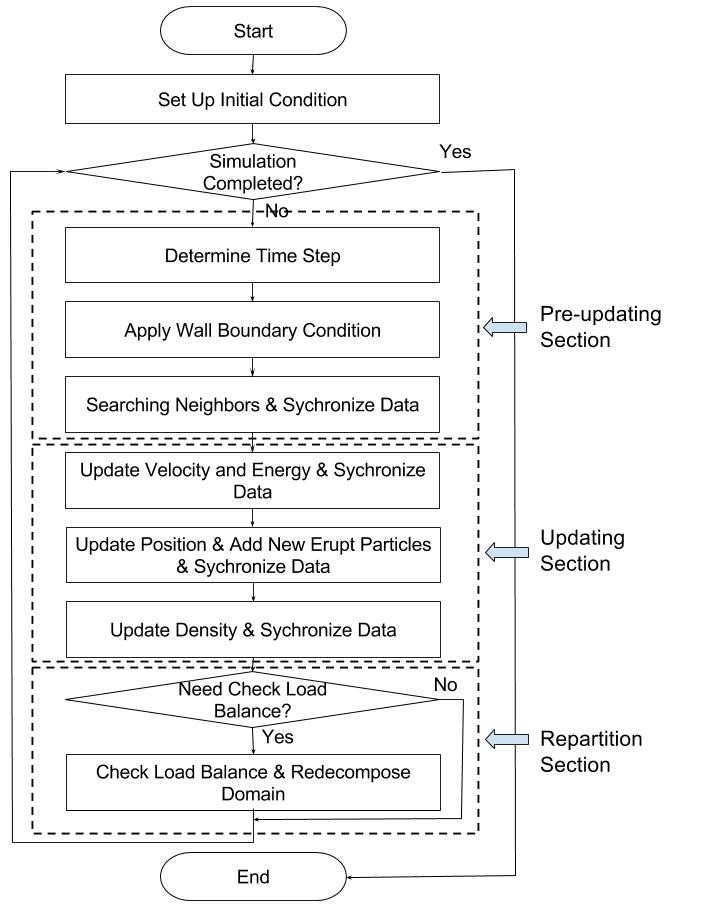
\includegraphics[scale=0.34]{Work_flow}
\caption{Basic work flow for SPH}
\label{fig:Work_flow}
\end{figure}
SPH is a meshfree, Lagrangian method. The domain is discretized by particles and the position of each particle is updated at every time step. The physical laws (such as conservation laws of mass, momentum and energy) written in the form of partial differential equations need to be transformed into the Lagrangian particle formalism of SPH. Using a kernel function that provides the weighted estimate of the field variables in the neighborhood of a discrete point (particle), the integral equations are evaluated as sums over neighbor particles. Only particles located within support of kernel function will interact. Thus, physical properties (position, density, velocity, internal energy, pressure) are updated based on its neighbors. So a neighbor search needs to be carried out before updating of physical properties. We use buckets which contain all particles associated with a sub-domain 
 and are kept fixed in time during the entire simulation, to reduce search cost (since search can now be restricted to only neighboring domains).
  Domain decomposition will be based on an SFC going through centroids of all buckets. A basic work flow of our SPH code is shown in figure \ref{fig:Work_flow}.\\
Particles need to be added and(or) removed during simulation of JPUE problems. Wall boundary conditions in SPH can be imposed either by adding a force term or using ghost particles. We adopt the latter one in our simulation. As our computational domain will be adjusted during simulation, wall ghost particles need to be added during simulation. New particles also need to be added for the eruption boundary condition. 
We will describe in this section   strategies which satisfies these requirements.
\subsection{SFC based indexing}
Our data structure starts from assigning each particle and bucket an identifier, we refer to it as key, which should be unique throughout simulation. The key for a bucket is determined by centroid coordinates of the bucket while the key for a particle is determined by adding coordinates and adding time step of the particle. The map from coordinates to key is based on SFC.\\
The SFC \cite{sagan2012space} maps n-dimentional space to a one dimentional sequence. The standard procedure for obtainning SFC is: 
\begin{itemize}
\item Scale coordinates into $[0,1]^n $ based on maximum and minimum coordinates of the computational domain: $\textbf{X}^\prime \rightarrow \textbf{X}$
\item Compute $k_r = h_n(\textbf{X})$. Where $h_n$ is the map $h_n: [0,1]^n \rightarrow [0,1]$. 
\item Convert $k_r$ to integer $k$ by multiplying $k_r$ with a very large number and removing decimal part.
\item All keys are sorted to form a sequence which is SFC. The SFC represents a curve passing through all particles (or centroid of buckets).
\end{itemize}
%In the following sections, the physics and SPH implementation of inject flow problem is given, then 
\begin{figure*}[!t]
\centering
\subfloat[SFCs passing all particles and buckets]{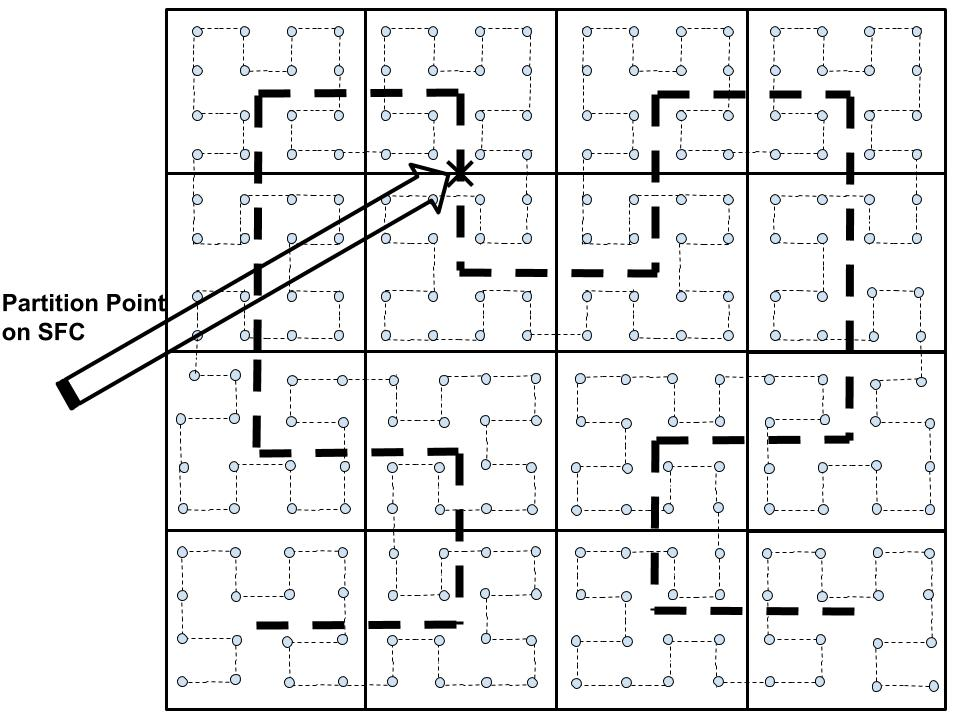
\includegraphics[scale=0.20]{SFC_particles_buckets}}
\label{fig:SFC_particles_buckets}
\hfil
\subfloat[Domain decomposition based on SFC of buckets]{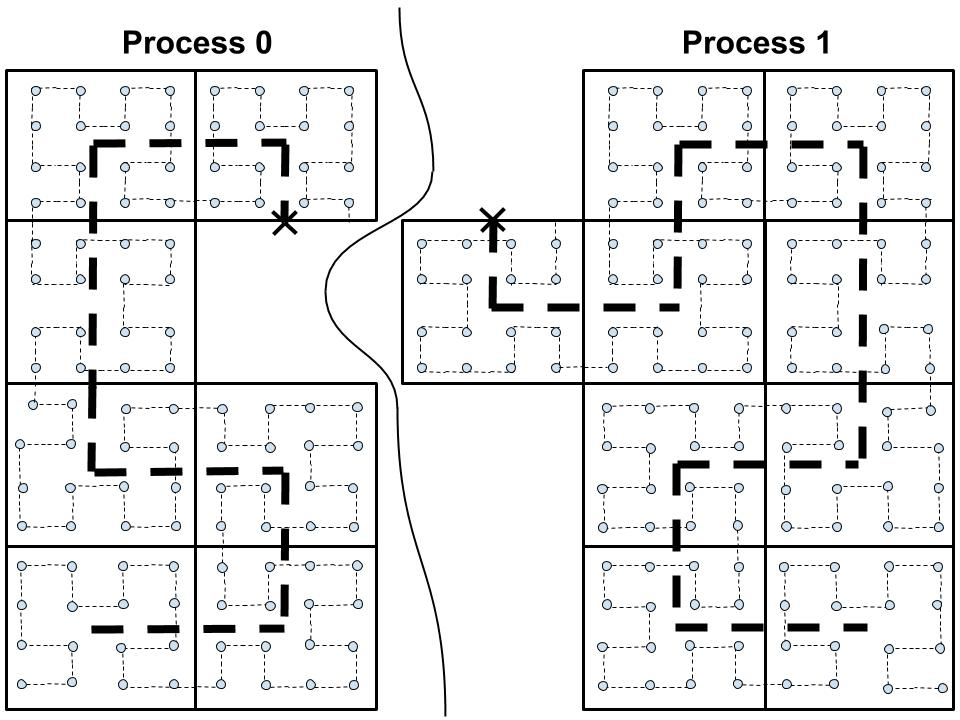
\includegraphics[scale = 0.22]{SFC_particles_buckets_partition}}
\label{fig:SFC_particles_buckets_partition}
\caption{Spcace filling curve orderings of buckets and particles within the buckets}
\label{fig:SFC_domain_decomposition}
\end{figure*}
Scheme for constructing the map $h_n$ can be found in \cite{patra1995problem}. These keys denote a simple addressing/ordering scheme for the data and computations, i.e., a simple global index space for all the objects.\\
SFC-based indexing scheme can guarantee uniqueness of particle identifier only in simple scenarios when particles are added once while setting up initial condition. In some situations, new particles need to be added while simulation. For example, new particles need to be added at the bottom of the eject vent for JPUE simulation. To distinguish particles added at the ``same place" (the small area, all points within which will be mapped to the same $k$.) at different time steps, we extend the SFC-based key to time-dependent SFC based key by including date of birth of particles into the key. The time-dependent SFC based key can be written as: $[k,t]$, where $t$ is the time step. The map $h_n$ will become:
\begin{equation}
h_n: [0,1]^n \times \textbf{T} \rightarrow [0,1] \times \textbf{N}
\end{equation}
Where $\textbf{T} \subset [0,\infty)$ is the time step dimension, $\textbf{N}=\lbrace 0, 1, 2, 3...\rbrace$.
To guarantee locality, sorting of particle keys is majorly based on $k$, that is to say, particle with smaller $k$ always comes before particles with larger $k$. For these particles have the same $k$, ordering of them will depend on $t$. Figure \ref{fig:SFC_particles_buckets} shows SFC ordering of buckets and particles in buckets. 
Several features of such indexing scheme are suitable for SPH:
\begin{itemize}
\item Guarantee uniqueness of keys.
\item Key of each object is generated purely based on its own coordinates. When add new objects on different processes, key of each object can be generated fast and independently.
\item Objects that locate closely in the Euclidian space will also be close to each other in the one dimensional SFC key space in the mean sense. Since SPH particles only interact with its neighbors, geometric locality can be exploited for efficient storage and retrieval of bucket and particle data.
\item This type of key effectively generates a global address space. Globality of key and conservation of locality make it easy to partition the sorted key sequence and obtain a decompositiion of the problem.
\end{itemize}
What we need to emphasize here is that in theory motion of particles will destroy locality established based on initial coordinates of particles. However, as particles are moving fairly regularly in a JPUE, the locality of most of particles should still be conserved during simulation.
%If we can design a re-numberring method which is computationally cheap, we can restore the locality.
\subsection{Data structure}
\subsubsection{Particle and bucket}
The most basic data structure of SPH are particle, for problem discription, and bucket, for neighbors searching and domain decomposition. Both are defined as classes in C++. Infomation that contained in particle class can be categorized into six categorise: ID(the key), affiliate(rank of the process that the particle belongs to), primitive variables (variables show up as unknows in governing equations, eg. density, velocity, energy), secondary variables (properties that can be computed from primitive variables, they are stored to avoid repeatedly computing, eg. pressure, temperature ect.), flags (indicators, such as indicator for ghost particle and real particles, indicator for particles of different phases ect.) and neighbor infomation (it is a vector of particle keys in our application). Similarly,  Infomation that contained in bucket class can also be categorized into different categorise: ID(the key), affiliate(rank of the process that the bucket belong to), domain information (maximum and mimnum coordinates, boundary infomation), flags (indicators, such as indicator for guest and non-guest, indicator for active and inactive), neighbor infomation (keys of 27 neighbor buckets for three dimension and keys of 9 neighbor buckets for two dimension including its own key) and possessed particles. Objects defined based on these two classes are then accesse through hash tables.
\subsubsection{Hash table and hash confliction}
As discussed at the beginning of this section, implementation of SPH in more realistic scenarios requires dynamic memory management and flexible data access. One of the fundemental data structures that satisfy such requirement is hash table. Another option is B-tree. We adopt hash table. An implementation of B-tree under a similar situation for mesh based methods can be found in other papers(eg.\cite{patra2003data}).\\
Hash table, which is divided into slots, are array based data structure. Based on the key, the address-calculator(hashing) function determines in which slot the data should be stored. The hashing function maps from key to the slot index:
\begin{equation}
slot\,index = hash(key)
\end{equation}
The hash table has O(1) data accessing, adding and deleting properties when there is no confliction. How many conflictions will happen depends on both distribution of keys in the key space and size of the hash table. As the distribution of keys is determined by particles' initial locations (or centroids of buckets), the hash table size is under our control. We can use very large hash table to minimize hash confliction on the expense of sparse data distribution which will lead to high cache missing and low memory efficiency. Or oppositely, we can use smaller hash table size to obtain high memory efficiency on the expense of having more hash conflictions. Abani\cite{patra2003data} did numerical experiments to examine
the e€ffect of the table size on the di€erent data management operations.\\
 %We should also do some experiment to optimize our hash table size.
One way to handle hash confliction is using an additional sorted vector attached to the hash table. When several keys hash to the same slot, a vector will be created. The vector is sorted based on keys so that a binary search can be used to find the correct position for adding, deleting or retrievaling . Another option to handle hash confliction is using an additional link list which is more flexible in memory allocation. The average time complexity of binary search is O(log n) while that for linear search based on link list is O(n). However, accessing efficiency of link list is much lower than array based data structure, especially when the link list becomes longger. Choosing of proper way to handle hash confliction greatly depends on the problem itself. For the test problem in this paper, successively adding of particles at the bottom of the eject vent will lead to hash confliction of many particles, which implies a long link list. But considering the very long conflictions only occur on several slots among millions (see figure \ref{fig:Particle_adding_with_link}), we still choose the link list to handle hash confliction. This decision was made based on numerical experiments.\\
\subsubsection{Hash function}
\begin{figure}[!t]
\centering
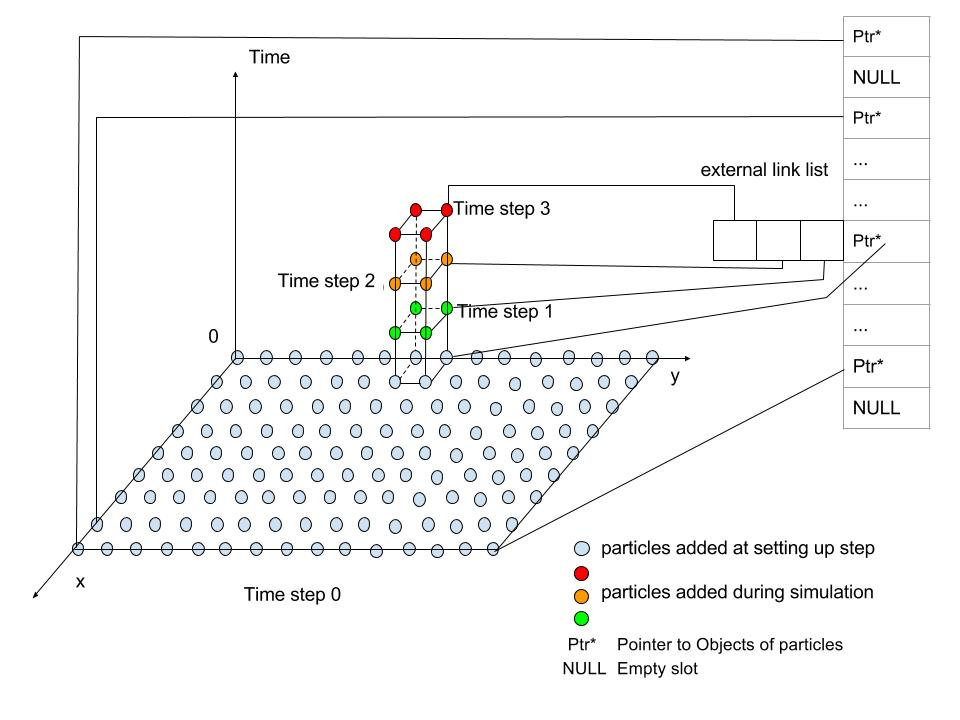
\includegraphics[scale=0.255]{Particle_adding_with_link}
\caption{Ununiform distribution of particles in the $[0,1]^n \times \textbf{T}$ space due to adding of new particles at a small portition of the domain, pointer to these new particles will be stored in external link list.}
\label{fig:Particle_adding_with_link}
\end{figure} 
For time-independent keys, the hash function can be a simple function like:
\begin{equation}
\label{eq:hash_function}
\begin{split}
Slot\,Index= &\frac{Key - Min\,Key}{Max\,Key - Min\,Key} \\
& \times Hash\,Table\,Size 
\end{split}
\end{equation}
One natural way to hash time-dependent SFC based key $[k,t]$ is to convert the two elements in the key into one number taking $k$ as the higher digit and $t$ as the lower digit of the large number. However, for JPUE simulation, even though ghost particles for wall boundary condition and pressure boundary condition also need to be added during simulation, places for adding of these two types of ghost particles are previsouly empty area. Only ghost particles for eruption boundary condition will be successsively added at the same place: bottom of the vent. That is to say, particles are distributed ununiformly in the $[0,1]^n \times \textbf{T}$ space as shown in figure \ref{fig:Particle_adding_with_link}. To avoid ununiform, very sparse hash table and conserve locality of SFC, we only plug the first number, $k$, of the key, $[k,t]$, into the hashing function, equation (\ref{eq:hash_function}). 
\subsection{Load balancing strategy}
\subsubsection{Weighted work load}
Particles used in the test problem can be categorized into four types based the particle-type-flag: real particle, wall ghost particle, pressure ghost particle and eruption ghost particle. Ghost particles are for imposing of corresponding boundary conditions (see figure \ref{fig:Involved_initial}). As different types of particles involve different amount of computational work, shown by table \ref{tab:Computational_cost_particles} and table \ref{tab:Computational_cost_steps}, we assign different work load weight for different types of particles based on profilling data. Instead of simply using number of contained particles as work load for bucket, work load of each bucket is determined by summing up work load weight of all particles within the bucket. The SFC sequence passing through centroids of all buckets now becomes a weighted sequence. Domain decomposition will conducted based on the weighted SFC of buckets.\\
\begin{table}[t!]
  \renewcommand{\arraystretch}{1.2}
  \centering
  \caption{Computational Cost Per Particle for Different Steps}
  \label{tab:Computational_cost_steps}
  \begin{tabular}{|c|c|c|}
    \hline
    Step & Cost ($ms$) & Abbreviation\\
    %\hhline{|=|=|=|}
    \hline
    neighbor search & 0.41 & NS\\
    \hline
    update momentum and energy & 0.70 & UPME\\
    \hline
    update density & 0.42 & UPD\\
    \hline
    update position & 0.02 & UPP\\
    \hline
    velocity filtering& 0.43 & VF\\
    \hline
    apply wall bc & 0.75 & WBC\\
    \hline
  \end{tabular}
\end{table}
\begin{table}[t!]
  \renewcommand{\arraystretch}{1.2}
  \centering
  \caption{Computational Work Load for Each Type of Particle}
  \label{tab:Computational_cost_particles}
  \begin{tabular}{|c|r|r|r|r|r|r|r|}
    \hline
    Particle type & NS & UPME & UPD & UPP &VF &WBC &Total\\
    \hline
    %\hhline{|=|=|=|=|=|=|=|=|}
    Real & Yes & Yes & Yes & Yes & Yes & No & 2.00\\
    \hline
    wall ghost & No & No & No & No & No & Yes &0.75\\
    \hline
    eruption ghost & No & No & No & Yes & No & No & 0.02\\
    \hline
    pressure ghost & No & No & No & No & No & No & 0.00\\
    \hline
  \end{tabular}
\end{table}
\subsubsection{Domain decomposition and dynamic load balancing}
Domain decomposition will be conducted based the weighted SFC of buckets. Figure \ref{fig:SFC_domain_decomposition} shows how domain is decomposed based on partition of SFC of buckets. The particles are automatically split into several groups along with buckets that contain them. As SFC of buckets is a curve in the three dimensional space, partition of this curve will automatically lead to 3D domain decomposition. A 2D domain decomposition based on SFC of footprint buckets projected by three dimensional buckets was adopted by Dinesh\cite{kumar2013parallel}. A comparision of the scalability of these two schemes (see figure \ref{fig:2D_vs_3D_efficiency}) confirms that 3D domain decomposition is a better choice when processes number is larger. 
%Some parallel implementations of SPH use 2D decomposition \cite{kumar2013parallel} even 1D decomposition \cite{marrone2012study, cherfils2012josephine}.  
%In our current implementation, the domain is partitioned only in $x-y$ plane. A two dimensional footprint of the three dimensional domain(as well as buckets) is generated by projecting. 
%SFC for the two dimensional footprint is partitioned for domain decomposition. The work load of each object on the SFC of footprint buckets in $x-y$ plane will be the summation of work loads of all buckets above the footprint. 
Movement of particles, adding of new particles, adjusting of domain will lead to important load imbalance between processes. To handle this, computational load is monitored at a given interval (The interval is optimized based on numerical experiments). And repartitioning is carried out when load imbalance is larger than a given tolerance.
\\
As some of the neighbor particles reside in other
partitions. A set of “guest” particles and buckets are used to synchronize data across partitions. To minimize communications, data is synchronized only where needed, using non-blocking MPI communications. 
\section{Adjusting of Domain During Simulation}
%SPH particles can be viewed as discretization points\cite{diltsg1999moving}. 
As a Lagrangian method, SPH is able to automatically adjust computational domain as the postition of the dicretization points are updated at every time step. However, for JPUE simulation, where some fluid ejects into stationary fluid and get mixed due to turbulence, the domain-adjusting feature of SPH will gone. Because the whole domain, which occupied by stationary fluid before ejected fluid reaching there, has to be discretized at the very beginning of simulation. A lot of CPU time will be spent on computing of "stationary" particles. It is pure wasting of computational resources. If simulating of stationary particls can be avoided, the computational cost will be reduced greatly. To the best of the author's knowledge, no implementation of SPH has the feature of adjusting computational domain based on simulation. We propose a simple strategy to add such feature in our code with low computational cost. We add a scan function to monitor the most outside layer of the domain. When the ejected fluid reaches the boundary of the current domain, ghost particles (for pressure boundary condition) will be turn to real particles and then add new ghost particles for pressure boundary condition. The original work flow (see figure \ref{fig:Work_flow}) is modified to enable such feature (see figure \ref{fig:Work_flow_adjust}).\\
\begin{figure}[!t]
\centering
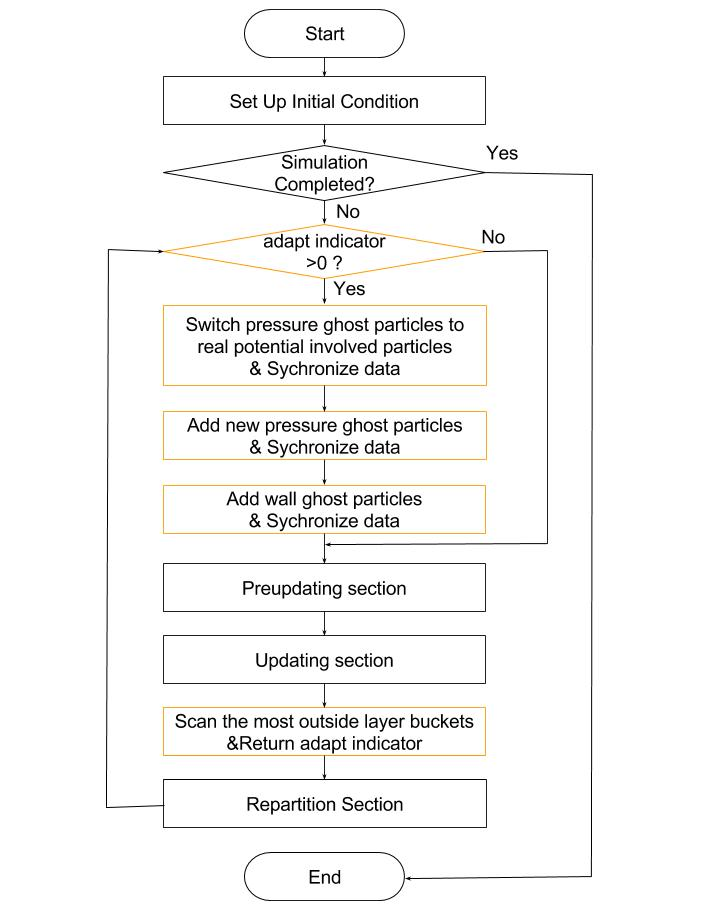
\includegraphics[scale=0.33]{Work_flow_adjust}
\caption{Work flow that enables domain adjusting feature}
\label{fig:Work_flow_adjust}
\end{figure}
The start point of adding adjusting feature is adding a flag, which we refer to as involved-flag, into particle class. Particles are categorized into three groups based on the value of the involved-flag: involved (involved-flag=2), potential involved (involved-flag=1), and not involved(involved-flag=0). The involved particles are particles that have already been involved in eject mixing. The potential involved particles are particles that have not been involved in eject mixing but adjecent to involved particles. So they will be involved in the near future. These not involved particles are particles that far away from the eject source and are still at the initial state. For these not involved particles, it is meaningless to update its physical properties. As a consequence, searching for neighbors and data communitation for these particles are also unnecessary. That is to say, only potential involved and involved particles need to be simulated.
As simulation goes, the ejected fluid will reach larger area and more and more particles will be influenced. When originally stationary air is influenced by erupted material, the mass fraction of the erupted material will increase from zero to a positive value. So we can determine whether a particle is involved or not based on whether the mass fraction of that particle is larger than a given threshold (10e-5 in our simulation). Other physical properties, such velocity, can also serve as alternative "swich criteria".\\
\begin{figure*}[!t]
\centering
\subfloat[Computational domain at $t=t0$]{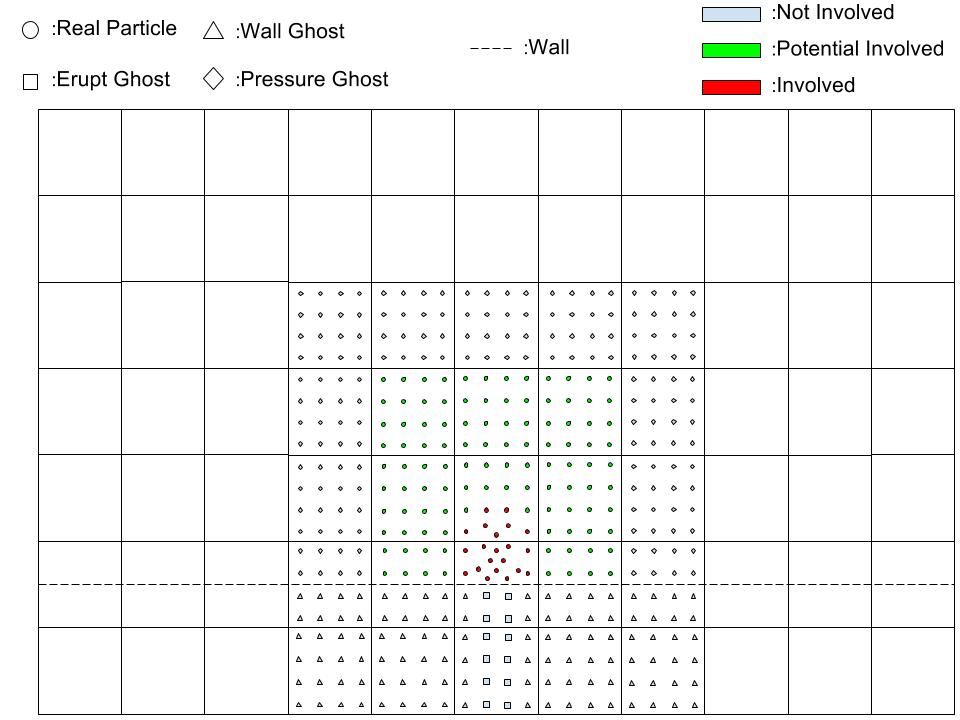
\includegraphics[scale=0.24]{Involved_initial}}
\label{fig:Involved_initial}
\hfil
\subfloat[Computational domain at $t=t0 + \delta t$]{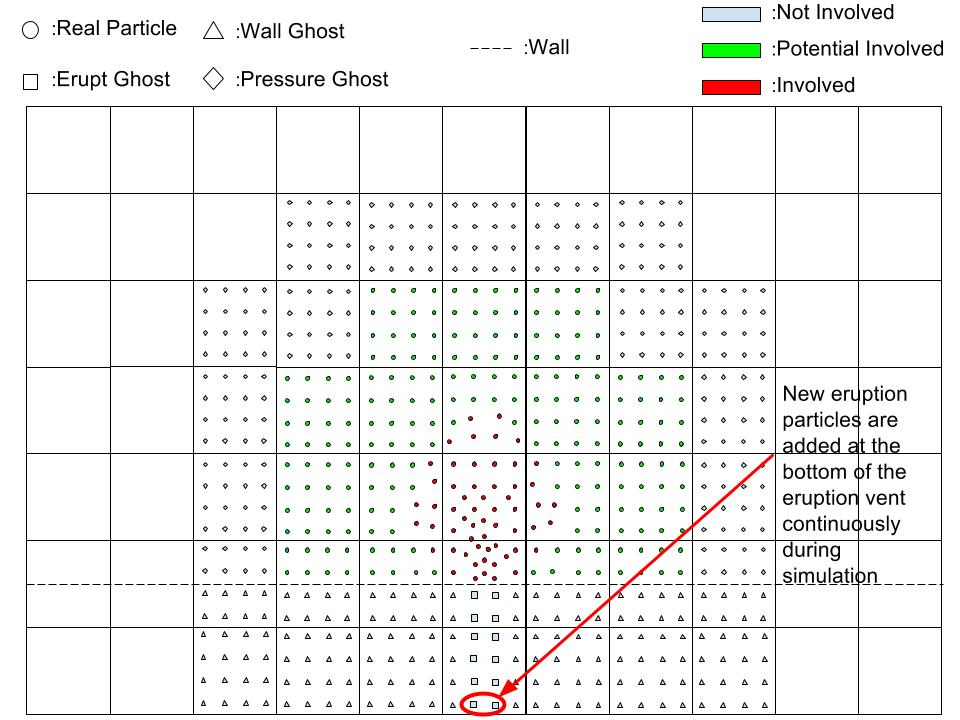
\includegraphics[scale = 0.24]{Involved_domain_adjusting}}
\label{fig:Involved_domain_adjusting}
\caption{Domain adjusting based on Involved flag of particles}
\label{fig:Domain_adjusting}
\end{figure*}
A has-involved-flag is added to bucket class, too. Buckets are then categorized into 3 types based on particles they contain: has involved (has-involved-flag=3), has potential involved(has-involved-flag=1) and has no involved (has-involved-flag=0). Bucket that has any involved particle will be set to be has involved (has-involved-flag=3). And its neighbor buckets that do not contain any involved particle will be set to be has potential involved. 
All particles in has involved buckets or has potential involved buckets will be set to be potential involved except for involved particles. There are two situations that will switch a has potential involved bucket to be a has involved bucket. First, when a involved particle enters a has potential involved bucket. Second, when mass fraction of a particle (It should be a potental involved particle) exceeds the threshold, this particle will turn to a involved particles and if this is the first involved particle in the bucket, the bucket will turn from a has potential involved bucket to a has involved bucekt.\\
The most outside buckets layer of all has potential involved buckets will be scaned every time after updating. If any of these buckets becomes has involved, the domain will be enlarged by turnning the pressure ghost particles to real particles and switching involved-flag from 0 to 1. Also, the buckets that originally contain pressure ghost particles will become has potential involved. New pressure ghost particles and wall ghost particles will be added around the adjusted domain.
This domain adjusting process is shown in figure \ref{fig:Domain_adjusting}.
The work flow with domain adjusting is in figure \ref{fig:Work_flow_adjust}\\
For the test problem in this paper, the volcanic plume will finally reach to a region of $[-10km \,\,\, 10km] \times [-10km\,\,\,10km] \times [0km\,\,\,20km]$ after around 300 seconds of eruption. When numerical simulation goes up to 90 seconds, the plume is still within a region of $[-3km\,\,\,3km] \times [-3km\,\,\,3km] \times [0km\,\,\,6km]$. This implies that adjusting of domain can avoid computing large number of uninfluenced air particles, especially for the beginning stage of simulation. Numercial test shows that simulation time of the test problem is reduce to $\frac{1}{4}$ of original simulation time when we adopt the domain adjusting strategy in our code.
\section{Numerical Test}
As we are targeting at developing data management and paralell strategies for more complicated implementations of SPH which demmand quick and flexible data access, delete and add. The test problem should have such demand. Volcanic eruption which is essentially a mutilple phases, turbulent, ejection mixing flow accompanied with microphysics processes requires more flexibile data management. We adopt a two phase volcanic plume model\cite{suzuki2005numerical} as our test problem. In this model, one phase is air while another phase is ejected material.
\subsection{Governing equations\cite{suzuki2005numerical} and boundary conditions}
Based on Navier-Stokes equations and several simplifications, the governing equations in Eulerian form are:
%the following assumptions are made:
%\begin{itemize}
%\item Molecular Viscosity is neglected since eddy viscosity due to turbulence is dominant. As heat conduction is much smaller than turbulent heat exchange \cite{oberhuber1998volcanic}, We only consider turbulent heat exchange.
%\item Erupted material consist of solid with different size and mixture of gas (various constituent) is assumed to be well mixed and behave like a single phase fluid (phase 2). Air (also a mixture of different gas) is assumed to be another phase (phase 1).
%\item We assume immediate thermodynamic equilibrium so that no separate energy equation is needed for each phase. As a result, there is only one energy equation for both phases and heat transfer effect between different phases will be ignored.
%\item We assume immediate dynamic equilibrium so that no separate momentum equation is needed for each phase. As a result, there is only one vector moment equation for both phases. Drag force term will not show up in the momentum equation as two phases always move with the same velocity.
%\item Because of above assumptions, all other micro-physics process (like phase change of $H_2O$, aggregation, decomposition, absorption of gas on the surface of solid, solution of gas into the liquid) and chemical process will not be considered in this model.
%\end{itemize}
%Finally the governing equations for this model in Eulerian form are:
\begin{equation}
\dfrac{\partial \rho}{\partial t} + \nabla \cdot (\rho \textbf{v}) = 0 \label{eq:gov-cs-rho}
\end{equation}
\begin{equation}
\dfrac{\partial \rho \xi}{\partial t} + \nabla \cdot (\rho \xi \textbf{v}) = 0 \label{eq:gov-cs-ks}
\end{equation}
\begin{equation}
\dfrac{\partial \rho \textbf{v}}{\partial t} + \nabla \cdot (\rho \textbf{v} \textbf{v} + p\textbf{I}) = \rho \textbf{g} \label{eq:gov-cs-v}
\end{equation}
\begin{equation}
\dfrac{\partial \rho E}{\partial t} + \nabla \cdot [(\rho E + p )\textbf{v}] = \rho \textbf{g} \cdot\textbf{v} \label{eq:gov-cs-e}
\end{equation}
$\xi$ is the mass fraction of ejected material.
$E = e + K $ is total energy which is summation of kinetic energy $K$ and internal energy $e$.
An additional equation is required to close the system. In this model, the equation for closing the system is an EOS:
\begin{align}
p = (\gamma_m - 1)\rho e \label{eq:EOS}
\end{align}
Where 
\begin{equation}
\gamma_m = R_m/C_{vm} + 1 \label{eq:gov-gm}
\end{equation}
\begin{equation}
Rm = n_gR_g + n_aR_a  \label{eq:gov-Rm}
\end{equation}
\begin{equation}
C_{vm} = n_s C_{vs} + n_g C_{vg} + n_a C_{va} \label{eq:gov-Cvm}
\end{equation}
\begin{equation}
n_a = 1 - \xi \label{eq:gov-na}
\end{equation}
\begin{equation}
n_g = \xi n_{g0} \label{eq:gov-ng}
\end{equation}
\begin{equation}
n_s = \xi - n_g \label{eq:gov-ns}
\end{equation}
Where, $C_v$ is specific heat with constant volume, $n$ is mass fraction, $R$ is gas constant. The subscription $m$ represents mixture of ejected material and air, $s$ is solid portion in ejected material, $g$ is gas portion in the ejected material and $a$ is air.\\
In current model the initial domain is a 3D box. The boundaries are categorized into eruption vent (a circle area at the center of the bottom), wall boundary (box bottom), pressure boundary (Other faces of the box).
At the vent, $T$, $\textbf{v}=\{0,0,150\}^T$, $p=1.01\times10^5 Pa$, $n_{g0}=0.05$ and mass discharge rate $\dot M$ is given. The radius of vent is determined from $\rho$, $\dot M$ and $\textbf{v}$.
Velocity is zero for non-slip wall boundary. We assume the boundary to be adiabatic and the heat flux is zero on the bounday. The pressure of the surrounding atmosphere is specified on pressure boundaries. Except for the pressure, density, velocity, and energy will depend on the solution. We adpot ghost particles to impose these different type of boundary conditions (see figure \ref{fig:Domain_adjusting}). 
\subsection{Discretized governing equations with SPH}
There are several review papers \cite{monaghan1992smoothed, monaghan2005smoothed, price2012smoothed, rosswog2009astrophysical, monaghan2012smoothed} which provide a pretty comprehensive view over SPH. We will not cover these basic theory of SPH in this paper.
The discretized governing equations with SPH are:
\begin{equation}
<\rho_a^a>=\sum m_b w_{ab} (h_a) \label{eq:gov-sph-d1}
\end{equation}
\begin{equation}
<\rho_i^{sg}>=\sum_j m_j w_{ij} (h_i) \label{eq:gov-sph-d2}
\end{equation}
\begin{equation}
\begin{split}
<\dfrac{d \textbf{v}_{\alpha}}{d t}>= &
-\sum_b [m_b (\dfrac{p_b}{\rho_b^2} + \dfrac{p_{\alpha}}{\rho_{\alpha}^2} + \Pi_{\alpha b}) \\ &\bigtriangledown_{\alpha}w_{\alpha b}(h_{\alpha})]
-\sum_j [m_j (\dfrac{p_j}{\rho_j^2} \\ & + \dfrac{p_{\alpha}}{\rho_{\alpha}^2} + \Pi_{\alpha j}) \bigtriangledown_{\alpha}w_{\alpha j}(h_{\alpha})]
+\textbf{g}
\end{split} 
\label{eq:gov-sph-v}
\end{equation}
\begin{equation}
\begin{split}
<\dfrac{d e_{\alpha}}{d t}>=&
 0.5\sum_b [m_b \textbf{v}_{\alpha b}(\dfrac{p_b}{\rho_b^2} + \dfrac{p_{\alpha}}{\rho_{\alpha}^2} + \Pi_{\alpha b})\\ & \bigtriangledown_{\alpha}w_{\alpha b}(h_{\alpha})]
+0.5\sum_j [m_j \textbf{v}_{\alpha b}(\dfrac{p_j}{\rho_j^2} \\ & + \dfrac{p_{\alpha}}{\rho_{\alpha}^2} + \Pi_{\alpha j}) \bigtriangledown_{\alpha}w_{\alpha j}(h_{\alpha})]
\end{split} 
\label{eq:gov-sph-e}
\end{equation}
Where
$\rho_a^a$ is density of phase 1 (air).
$\rho_i^{sg}$ is density of phase 2 (erupted material).
$\rho=\rho^a + \rho^{sg}$ is density of mixture of phase 1 and phase 2.
\begin{equation}
\textbf{v}_{\alpha b}=\textbf{v}_{\alpha}-\textbf{v}_b
\end{equation}
\begin{equation}
\textbf{v}_{\alpha j}=\textbf{v}_{\alpha}-\textbf{v}_j
\end{equation}
$w_{ab} (h_a)= w(\textbf{r}_a-\textbf{r}_b,h_a)$ is smoothing kernel.
%$\bigtriangledown_{\alpha}w_{\alpha j}(h_{\alpha})$-->need double check
$\Pi$ is artificial viscosity term \cite{monaghan1992smoothed}.
Index $a$, $b$ is for phase 1.
Index $i$, $j$ is for phase 2.
Index $\alpha$, $\beta$ can be index of either phase 1 or phase 2.
The position of each particle is updated according to the following equation.
\begin{align}
\dfrac{d \textbf{r}_a}{dt} = \textbf{v} \label{eq:gov-update-pos}
\end{align}
Free surface flow are in nature turbulent. We adopt $SPH-\varepsilon$ method developed by Monaghan\cite{monaghan2011turbulence} to capture turbulence in the plume. This will result to a filtered velocity for position updating and additional turbulent terms in momentum and energy eqution.
\subsection{Solver performance}
\begin{figure}[!t]
\centering
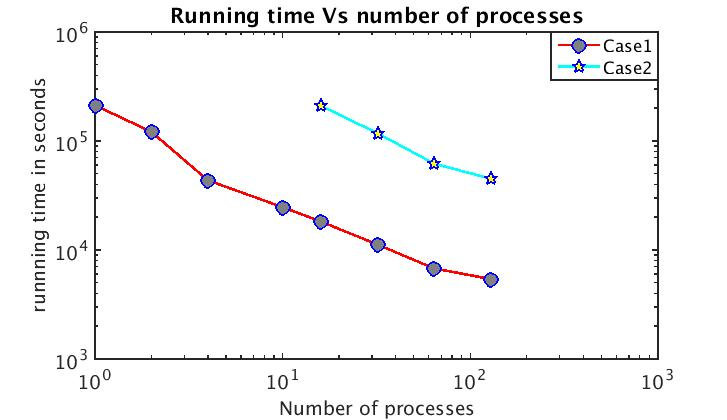
\includegraphics[scale=0.33]{2cases_time}
\caption{Excuting time of test case 1 and test case 2}
\label{fig:2cases_time}
\end{figure}
%
\begin{figure}[!t]
\centering
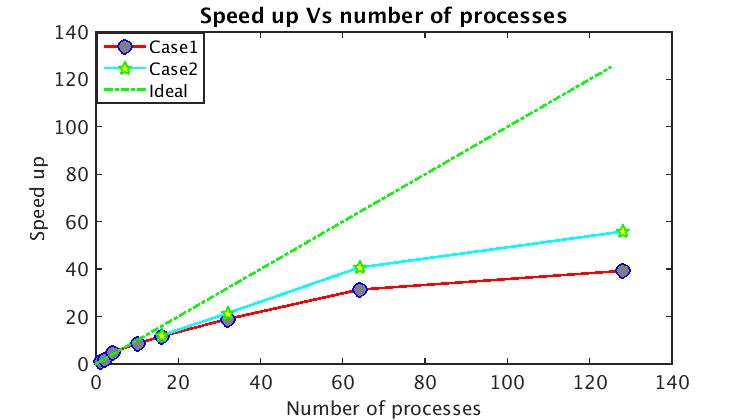
\includegraphics[scale=0.33]{2cases_efficiency}
\caption{Influnece of total work load on strong scalability}
\label{fig:2cases_efficiency}
\end{figure}
%
\begin{figure}[!t]
\centering
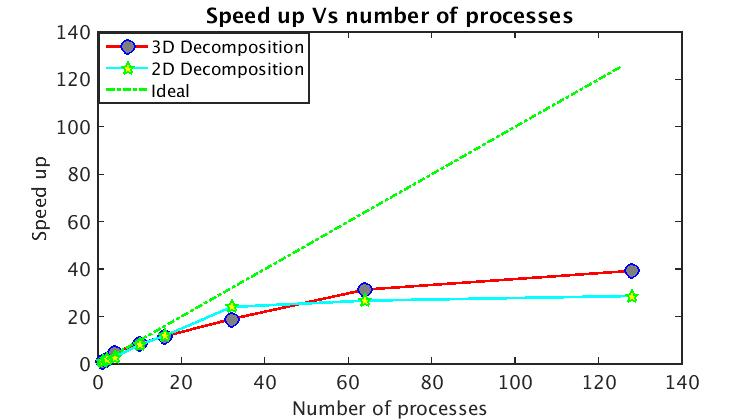
\includegraphics[scale=0.33]{2D_vs_3D_efficiency}
\caption{Strong scalability of 3D domain decomposition and 2D domain decomposition}
\label{fig:2D_vs_3D_efficiency}
\end{figure}
%
\begin{figure}[!t]
\centering
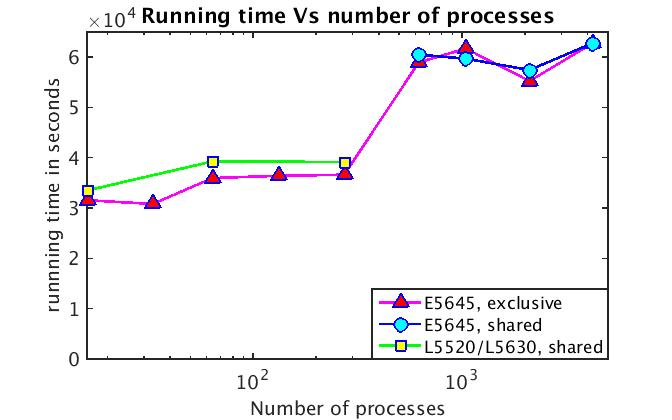
\includegraphics[scale=0.33]{weak_loglog}
\caption{Weak scalability test results}
\label{fig:weak_loglog}
\end{figure}
%Experiments have been carried out on the computational cluster of Center for Computational Research (CCR) at Buffalo. 
The initial domain is $[-4800m,4800m]\times [-4800m,4800m] \times [0m, 6000m]$, with smoothing length (we set initial intervals between particles equal to smoothing length) equals to 200m and 100m respectively for test case1 and test case2. The computational work load of test case 2 is 8 times of that of the test case 1. The simulations run for 20s physical time. The consumed time and speed up are shown in figure \ref{fig:2cases_time} and \ref{fig:2cases_efficiency}. Linear speed up is observed when number of processes is smaller than 16. Test case2 shows better speed up than test case1 which implies that the overhead of strong scalability can be increased by increasing total amount of work load. We also compared the performance of 2D domain decomposition and 3D domain decomposition. As shown by figure \ref{fig:2D_vs_3D_efficiency}, 2D domain decomposition shows a little bit better speed up than 3D domain decomposition for 32 processese. This can be explained by the fact that 2D domian decomposition can get more regular subdomain and as a results, need less communication. When number of processes increase, it becomes harder for 2D decomposition to balance workload, that is why 3D domain decomposition has better speed up for processes number equals to 64 and 128. The weak scalability test is conducted with the same initial domain and various smoothing length. Each simulation runs for 400 loops. The average number of real particles of each process keep constant. As shown in figure \ref{fig:weak_loglog}, simulation time increases pretty slowly when number of processes is larger than 132. the relative sharp increase in simulation time from 32 processes to 132 processes might cause by a increase of number of neighbor processes. 
%That can be explained by the fact that the total number of footprint buckets in x-y plane is 64 in the test case.
%When we request 128 processes, 64 processes will be totally idle at the beginning. As simulation goes, the domain will expand and more and more idle processes will start getting tasks. That's why we still get some speed up when number of process is 128. 3D domain decomposition is able to divide the work load in a more flexible way and achieve better strong scalability.
\section{Conclusion}
We developed data management strategies for parallel implementation of SPH method using MPI standard to simulate complicated problems, such as JUPE, which requires flexible and fast data retrievalling, adding and deleting. Neighbors searching and domain decomposition is based on background grid which overlaps the domain and keep stationary during simulation. SFC based index scheme, which provides a global numberring methodology which is purely coordinates dependent, is adopted to give each bucket an unique identifier. A time dependent key which is also based on SFC is used as identifier for particle. 
Hashtables with external link list are adopted for accessing particles and buckets data. Based on weighted particle work load, a dynamic load balance strategy is developed by checking load balance and redecomposing the domain at an optimize interval. The performance of the code was further improved to several times faster by adjusting computational domain according to progress of simulation. 
Scalability tests on our code shew acceptable strong scalability and good weak scalability. 3D domain decomposition provided better strong scalability than 2D domain decomposition when number of processes is larger.
% An example of a floating figure using the graphicx package.
% Note that \label must occur AFTER (or within) \caption.
% For figures, \caption should occur after the \includegraphics.
% Note that IEEEtran v1.7 and later has special internal code that
% is designed to preserve the operation of \label within \caption
% even when the captions off option is in effect. However, because
% of issues like this, it may be the safest practice to put all your
% \label just after \caption rather than within \caption{}.
%
% Reminder: the "draftcls" or "draftclsnofoot", not "draft", class
% option should be used if it is desired that the figures are to be
% displayed while in draft mode.
%
%\begin{figure}[!t]
%\centering
%\includegraphics[width=2.5in]{myfigure}
% where an .eps filename suffix will be assumed under latex, 
% and a .pdf suffix will be assumed for pdflatex; or what has been declared
% via \DeclareGraphicsExtensions.
%\caption{Simulation results for the network.}
%\label{fig_sim}
%\end{figure}

% Note that the IEEE typically puts floats only at the top, even when this
% results in a large percentage of a column being occupied by floats.


% An example of a double column floating figure using two subfigures.
% (The subfig.sty package must be loaded for this to work.)
% The subfigure \label commands are set within each subfloat command,
% and the \label for the overall figure must come after \caption.
% \hfil is used as a separator to get equal spacing.
% Watch out that the combined width of all the subfigures on a 
% line do not exceed the text width or a line break will occur.
%
%\begin{figure*}[!t]
%\centering
%\subfloat[Case I]{\includegraphics[width=2.5in]{box}%
%\label{fig_first_case}}
%\hfil
%\subfloat[Case II]{\includegraphics[width=2.5in]{box}%
%\label{fig_second_case}}
%\caption{Simulation results for the network.}
%\label{fig_sim}
%\end{figure*}
%
% Note that often IEEE papers with subfigures do not employ subfigure
% captions (using the optional argument to \subfloat[]), but instead will
% reference/describe all of them (a), (b), etc., within the main caption.
% Be aware that for subfig.sty to generate the (a), (b), etc., subfigure
% labels, the optional argument to \subfloat must be present. If a
% subcaption is not desired, just leave its contents blank,
% e.g., \subfloat[].


% An example of a floating table. Note that, for IEEE style tables, the
% \caption command should come BEFORE the table and, given that table
% captions serve much like titles, are usually capitalized except for words
% such as a, an, and, as, at, but, by, for, in, nor, of, on, or, the, to
% and up, which are usually not capitalized unless they are the first or
% last word of the caption. Table text will default to \footnotesize as
% the IEEE normally uses this smaller font for tables.
% The \label must come after \caption as always.
%
%\begin{table}[!t]
%% increase table row spacing, adjust to taste
%\renewcommand{\arraystretch}{1.3}
% if using array.sty, it might be a good idea to tweak the value of
% \extrarowheight as needed to properly center the text within the cells
%\caption{An Example of a Table}
%\label{table_example}
%\centering
%% Some packages, such as MDW tools, offer better commands for making tables
%% than the plain LaTeX2e tabular which is used here.
%\begin{tabular}{|c||c|}
%\hline
%One & Two\\
%\hline
%Three & Four\\
%\hline
%\end{tabular}
%\end{table}


% Note that the IEEE does not put floats in the very first column
% - or typically anywhere on the first page for that matter. Also,
% in-text middle ("here") positioning is typically not used, but it
% is allowed and encouraged for Computer Society conferences (but
% not Computer Society journals). Most IEEE journals/conferences use
% top floats exclusively. 
% Note that, LaTeX2e, unlike IEEE journals/conferences, places
% footnotes above bottom floats. This can be corrected via the
% \fnbelowfloat command of the stfloats package.

% conference papers do not normally have an appendix

% use section* for acknowledgment
\ifCLASSOPTIONcompsoc
  % The Computer Society usually uses the plural form
  \section*{Acknowledgments}
\else
  % regular IEEE prefers the singular form
  \section*{Acknowledgment}
\fi

Computational results reported here were performed at
the Center for Computational Research at the University at
Buffalo. This project is supported by Grants No. NSF
1131074 from the National Science
Foundation.


% trigger a \newpage just before the given reference
% number - used to balance the columns on the last page
% adjust value as needed - may need to be readjusted if
% the document is modified later
\IEEEtriggeratref{28}
% The "triggered" command can be changed if desired:
%\IEEEtriggercmd{\enlargethispage{-5in}}

% references section



% can use a bibliography generated by BibTeX as a .bbl file
% BibTeX documentation can be easily obtained at:
% http://mirror.ctan.org/biblio/bibtex/contrib/doc/
% The IEEEtran BibTeX style support page is at:
% http://www.michaelshell.org/tex/ieeetran/bibtex/
\bibliographystyle{IEEEtran}
% argument is your BibTeX string definitions and bibliography database(s)
%\bibliography{IEEEabrv,../bib/paper}
\bibliography{Reference}
%
% <OR> manually copy in the resultant .bbl file
% set second argument of \begin to the number of references
% (used to reserve space for the reference number labels box)
%\begin{thebibliography}{1}
%
%\bibitem{IEEEhowto:kopka}
%H.~Kopka and P.~W. Daly, \emph{A Guide to \LaTeX}, 3rd~ed.\hskip 1em plus
%  0.5em minus 0.4em\relax Harlow, England: Addison-Wesley, 1999.
%
%\end{thebibliography}


% that's all folks
\end{document}


